% This is the term paper for the CSCW class for which the tool Impact!
% was created and evaluated. This was done solely by Jordan Ell

\documentclass[conference]{IEEEtran}

\usepackage{graphicx}
\usepackage{amsmath}

\hyphenation{op-tical net-works semi-conduc-tor}

\begin{document}

%Paper title
\title{Creation of Developer Awareness Inside Changesets Using Method Hierarchy}

%Author block
\author{\IEEEauthorblockN{Jordan Ell}
\IEEEauthorblockA{University of Victoria,
Victoria, British Columbia \\ jell@uvic.ca}}

\maketitle

\begin{abstract}
Software systems have become larger over time, and as a result these system's number of developers
and technical dependencies between developers has also increased. With these expansions also
comes the increasing risk of a software change having an negative impact somewhere else inside
of the software system. Software failures are a multi-billion dollar issue faced by the industry and
while better form of testing and integration are helping to ensure a minimal number of failures, 
research to prevent failures caused by software changes is still a major concern. Numerous coordination
recommendation systems have been built which base there recommendations off of software dependencies,
but none focus on the impact dependencies of software changes. This paper describes how analysis
of software changes and the technical relationships they infer can be used to create awareness among
developers in order to avoid potential software failures. This awareness is presented using a web based
application which takes advantage of software hierarchy and developer code changes.
\end{abstract}

\section{Introduction}
Large software projects are often created using highly modular and reusable source code such as methods
and objects. The use of these methods and object creates a vast amount of technical dependencies between
these structures and can be in a wide variety of locations throughout a software project. This causes any
changesets of source code to have a rippling effect, or impact effect, across the rest of the project
~\cite{Acharya:2011:PCI}. The large the software project, the larger are these changes tend to impact
and cause a larger number of software failures inside the system during the project's life span
~\cite{Zimmermann:2008:PDU}. These observations of modular source code structure and the
technical dependencies that they infer open the door to types of dependency network analysis
in order to prevent software failures in a software system.\\

Technical dependencies are often used to predict software failures in builds or changesets of
a software system~\cite{Pinzger:2008:DNP, Zimmermann:2008:PDU}. Most pre-existing research
has focused on a very high level modular approach as either the binary or file level~\cite{Kim:2006:AIB}. 
These high level
modules are mostly studied for logical dependencies on which modules are changed together most
often. When files A and B are always changed together or binaries A and B then it is assumed that
when a changeset is committed to the source repository using on file or binary A then there is
a high chance of inducing a software failure~\cite{Beyer:2005:CSA}. These high level predictions are often not able to
provide any support to developers other than test focus or minor amounts of social
coordination recommendations.\\

Not only are technical dependencies a known way to prevent software failures, but as is the 
notion of awareness. Awareness is the ability to know and understand what actions
other members of a development team are taking. Through the notion of awareness, developers
are provided information on their development product from which they can deduce their
own social coordination actions. These actions can often lead to the prevention of software
failures or catch software failures in an early stage of life. One type of awareness is that of
workspace awareness which is up to the minute knowledge about other's interactions
with a workspace~\cite{Gutwin:1996:WAR, Gutwin:1996:USA}. This type of awareness can
often lead to high level details of a project.\\

Like technical dependencies, pre-existing workspace awareness tools also focus mostly on the high level
details of a project. Most awareness tools focus on the file level to let developers know who
is currently working on or viewing a file~\cite{Biehl:2007:FVD}. There have also been some applications which focus
on the lower modular levels of objects and methods but the information given about these
interactions is still only changing the module or viewing in most cases~\cite{Biehl:2007:FVD}.
These types of awareness
allow developers to get a sense of real time development but fail to show the full impact
of changes being made inside of a software system.\\

With the power of technical dependencies and awareness in software failure prediction and
prevention at high level modules, the question is posed:
"\textit{Is it possible to identify impact effects of code changes at low structural levels and can
these effects be used in an awareness tool to prevent software failures and induce social
coordination recommendations?}"\\

This paper will take the approach of discovering code change impact effects at the method
level of source code. The method level was chosen because of its usage across multiple
software languages as opposed to object which are only used in object oriented languages
such a C++ of Java.  Recent science suggest that exploration in an environment
is directed by the information that we have picked up~\cite{Neisser:1974:USE}. Thus, if we are able to relay
information to the developer at a method level, bug prevention at that level may
also be possible. Once code change impact effects are found at the method level, the 
linkage of technical dependencies to developers will be described. Finally, this paper will
describe how this newly acquired dependency information can be used to create an awareness
tool for developers in order to prevent software failures and create social coordination
recommendations between developers using an awareness tool.\\

This paper will also evaluate the end tool produced through developer interviews of teams
who have actually used the tool.  The evaluation will be followed up by a discussion of
the tools effectiveness and suggestions for future development and research.\\


\section{Creation of Awareness Tool}

The basis of the tool Impact is to create an information space which developers can see awareness information
based on the code they have written at the method level of source code. Impact will provide information to the
developer based on method ownership and those method's call hierarchies effected by changesets.  To preform
these actions, a two step approach will now be described. \\

\subsection{Extracting Technical and Developer Dependencies}
To extract the information needed for the Impact awareness tool, the source code repository must be queried to
extract information such as method ownership and method call hierarchies during a changeset. This information
will provide technical dependency edges between developers caused by changesets which can then be used as
awareness information and provided to the developers. \\

At each changeset, the method call graphs must be constructed. Method call graphs are a simple graph which uses
method declarations as nodes and method invocations as directed edges. To construct the call graphs, the source 
code repository (in this case Git) must be queried to obtain all source files of the project. Unlike Bodden's et al.
~\cite{Bodden:2003:HVJ}  approach of using byte code and whole projects, call graphs are built directly from source
code files inside of code changes, which does not have the assumption of being able to fully compile.
It is important not to require full project complication at each code change because it is an
expensive operation as well as code change effect may cause the project to be unable to compile.
Once all source files are
obtained, abstract syntax trees (AST) are then compiled for each file. The abstract syntax trees contain all information
in regards to the method call hierarchies of the project. From here, the call hierarchies can be constructed by simply
querying the ASTs in regards to method call structures. The method call graphs have now been constructed.\\

Once the method call graph has been constructed, the changeset can be used to identify the Impacted methods
of the changeset which will be used for developer awareness information. The Git repository now needs to be
queried in order to identify which methods have been changed by the changeset. This information can be 
extracted by using the "git diff" command. This command lists all information regarding files and lines
changed inside of a changeset. This information can then be put against the method call graphs as it is now 
known which lines of files, leading to which method, have been changed inside of the changeset. With each
changed method now found, a final query is made against the call graph to find those methods which invoke
the changed methods. These methods which invoke those changed will become the basis for the awareness
information to presented to developers. \\

Next, each invoking method inside of the call graph must be assigned weighted owners. The owners of a method are obtained
by using the Git repository. Git stores which developers have written which lines of code inside of a project, including
other information such as which changeset the line of code comes from and time and date. This information can be
retrieved by using the "git blame" command. To obtain weighted owners for each method a simple weight of number 
of lines written divided by total lines inside the method is given to each owner who is partially responsible for writing
each method. The weight method owners have now been obtained. \\

Between the method call graphs, identified changed and invoking methods of a changeset and their owners,
final developer network can now be constructed. This construction can be seen inside of Figure~\ref{fig:network}.
Here the method call graph between methods bar(), foo() and getX() has been constracuted with its owners
( Figure~\ref{fig:network} left hand side).
Inside of Carl's changeset, the function getX() has been modified. Since Impact is only interesting in developer
awareness and not method awareness, the network is simplified to involve only developers
( Figure~\ref{fig:network} right hand side). The awareness information is now ready to be presented to the
developers. \\

% Technical network figure
\begin{figure*}[tb!]
\centering
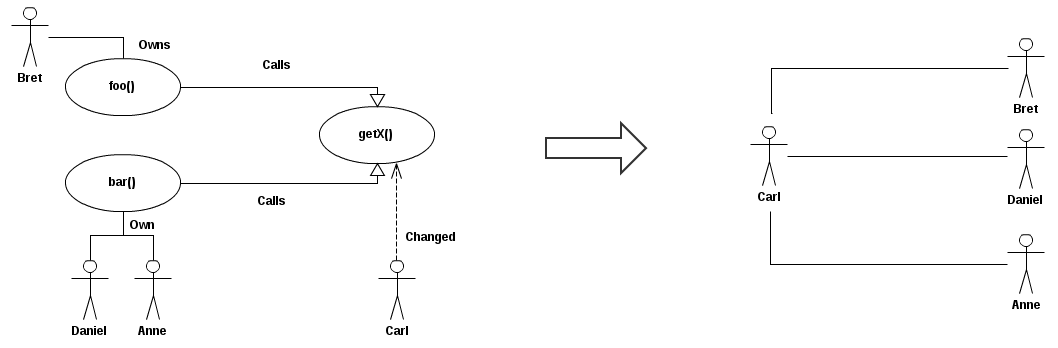
\includegraphics[width=0.9\textwidth]{images/TecNetwork}
\caption{A technical network with resulting developer network for a code change. Carl has changed method getX() which is being
called by Bret's method foo() as well as Daniel and Anne's method bar().\label{fig:network}}
\end{figure*}

\subsection{Providing Awareness Information}
For Impact to provide appropriate awareness information to the correct developer, three steps must be taken.
First the source code repository must be updated. Second the awareness information must be gathered from 
the repository. Lastly, the information must be stored in a database and presented to the developer in an 
appealing manner. \\

In order to update the code repository when new changesets are committed, a service hook must be used.
A service hook is a trigger stored on the project's central repository which sends information to an outside
server whenever activity with the central repository occurs (in this case a new changeset). A git hook is installed
on the project's central repository and hooked up to the Impact server being run. Once the Impact server 
receives the notification that a new changeset has been committed, Impact updates its local repository to
reflect this new changeset. From here the Impact tool proceeds to gather the awareness information needed
for the developers. \\

The awareness information is then gathered in the manner described in the previous subsection. Once the 
information has been gathered, it is stored inside of a local database on the Impact server for later use.\\

Now that the Impact server has the ability to gather and store information regarding the project's source code
repository, a front end must be used for developers to see the appropriate information. This front end
takes the form of a web application. Developers can visit the Impact server using a web browser in order to
see their awareness information. Developers are able to log into the Impact server using the same credentials 
as their source code repository and are then presented with RSS type feeds with awareness information.
The feeds can be used for tracking many different objects at the developers request, but the main purpose
is to display the awareness information gathered in the last subsection. This feed is called the Method Impact
feed and can be seen in Figure~\ref{fig:impact} as the left most feed. Here developers can see their methods
which have been impacted by other developer's changesets inside of the project. \\

The other types of feeds which are supported by Impact are Person and File feeds which can be seen as
the central and right most feeds respectively in Figure~\ref{fig:impact}.\\

%Impact figure
\begin{figure*}[tb!]
\centering
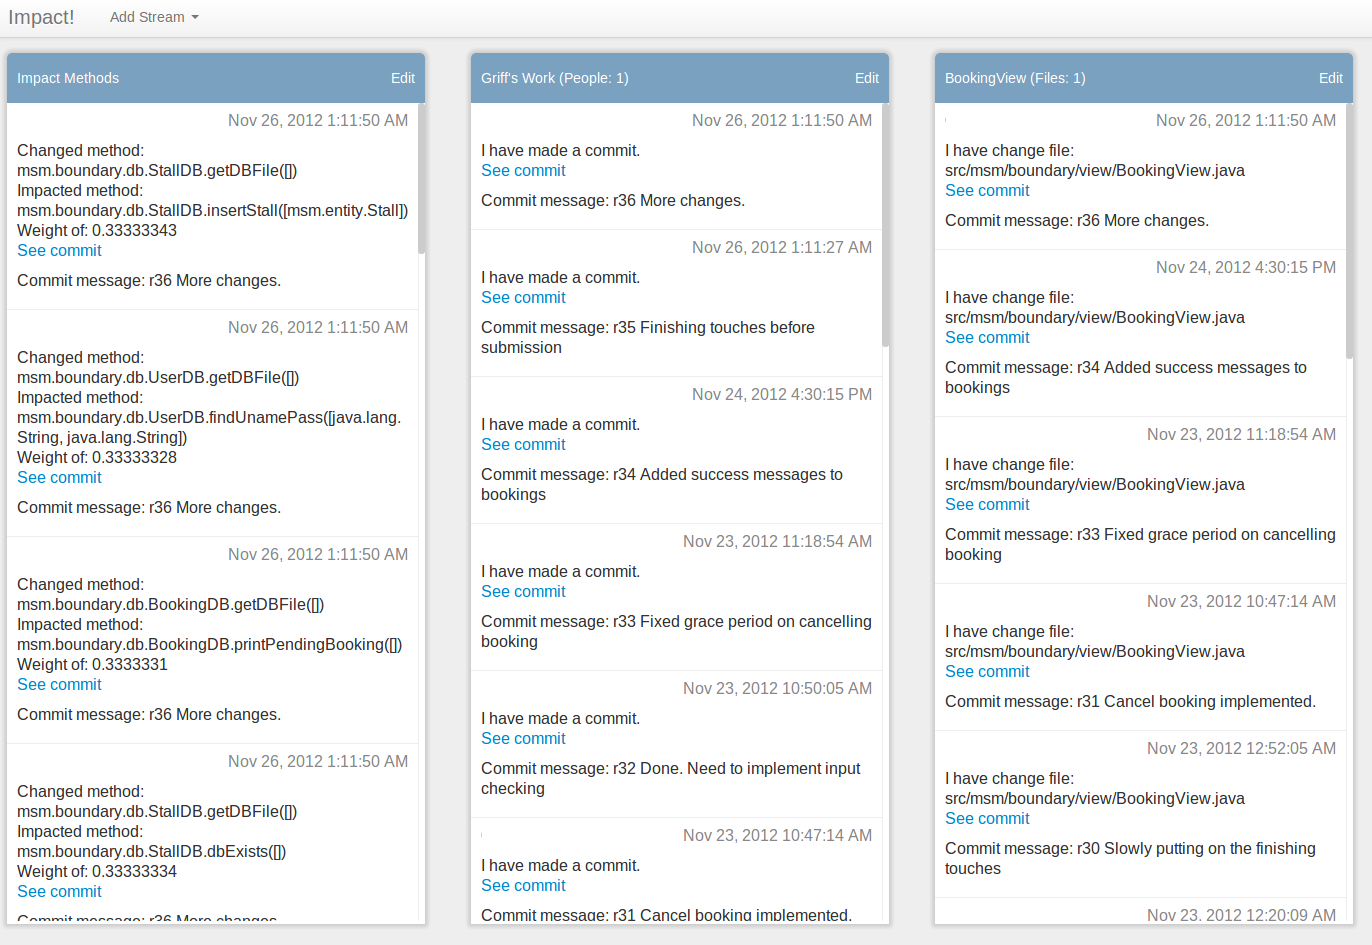
\includegraphics[width=0.9\textwidth]{images/ImpactDemo}
\caption{The tool Impact with developer names hidden.\label{fig:impact}}
\end{figure*}


\section{Evaluation}

\subsection{Participants}
In order to evaluate Impact, two case studies were used. The University of Victoria hosts an undergraduate
level class called Object Oriented Design (SENG 330) where students learn the practises of object oriented
programming languages and how design patterns can be used with these languages to achieve quality 
software applications. The course is taught with a hands on approach as student groups build a software
product over the course of the semester. Students go through all proper processes of building the product
such as requirements engineering, design, prototype/mock-ups, and final implementation. 
The final projects are presented at the end of semester. \\

A pitch for Impact was made in front of this class in order to request that teams use Impact as a tool during 
their development process. Two teams responded as willing participants for the use of Impact. Both teams 
had three members and were led by a core developer. \\

Team 1 was tasked with developing an arena bookings management system. The project was written in
Java and had a command line interface. The team was led by a 2nd year undergraduate student who was
also the core developer and backed up by two 3rd year undergraduates who also preformed minor
development. Team 1's lead developer Carl has had two years of development experience and is 
beginning to move into professional development.\\

Team 2 was tasked with developing a market management system. The project was written in Java
and used a Java Swing interface. The team was led by a 4th year undergraduate student who was
the sole developer of the project and also contained two 3rd year undergraduates. Team 2's lead
developer John has had 2 years of professional development experience and is involved in numerous
on going projects outside his professional career.\\

Each of the two teams was given an Impact server which was then used as a part of their development
process for the course project.

\subsection{Evaluation Strategy}
In order to evaluate the effectiveness of Impact in providing awareness information to the developers
on each of the two studied teams, semi-structured interviews were conducted with each of the team's
lead developers. A semi-structured interview was used as evaluating awareness applications is a
difficult task to approach with a formal structure. Questions were prepared ahead of time but, most
of the interviews ended up being spin off discussions from the original questions. Only the team's
lead developers were interviewed for multiple reasons. The first being these lead developers had the
most to benefit from the tool and had seen it in action most because of the larger amounts of
development done by these individuals. The second being these leads had the most external development
experience on their respective teams which allows them to approach the tool with knowledge of
other projects and its potential on them as well. The last being these developers produced most of
the source code for their respective projects which allowed them to use the tool more than the 
other members of their team.  \\

The interviews themselves focused on four areas of interest. The first being the developers background.
Establishing the interviewee as a competent developer with experience is crucial as the answers
provided about the tool need to be backed up by developer experience.  The second being determining
if bugs or problems arise in software these developers have worked on because of other developers
actions. These questions establish that Impact is attempting to solve a real world problem. This
is a crucial step in the interview which gives the tool legitimacy for future applications. The third
area of interest is understanding what types of actions other developers take which cause bugs
or unwanted processes in the developer's own code. These questions establish a domain of 
research. The hoping here is that the interviewees identify regions of source code which are
potentially harmful structures when changed by developers that can effect their own code. Impact
focuses on the method as the harmful structure. The final area of interest was a series of questions
which focused on conflict resolution. After the interviewee establish the existence of the problems
and provided a domain of knowledge, they were asked to explain how such conflicts were
discovered and resolved. \\

From the four areas listed above, it should be determinable whether or not Impact is a useful tool
without explicitly asking the developers. However, the developers were asked for their opinions 
on Impact as a tool for their team's development as well as its use in industry and what changes
they would make to the tool. \\


\section{Results}
This section will be broken up between in the responses of the two lead developers in regards to
the four areas of interview interest.

\subsection{Team 1 Lead Developer}
Team 1's lead developer, Carl, had a background of being a 2nd year computer science undergraduate
at the University of Victoria. He has been developing for just over 2 years but has yet to have real world
development experience although having had worked on several software projects outside of academia. \\

From the interview Carl had mentioned that he has faced numerous software bugs because of other changes
inside of the system. He has done bug fixing which he essentially related to fixing bugs caused by new
feature development which caused older code to fail. This establishes the fact that the problem Impact
is attempting to solve is a real world, the problem being other developers changesets effect other the
developer's own code in a negative way. In the third interview focus, Carl identified individual commits
as being a large contributor to producing bugs but more importantly he mentions that the source code
changes that occur as the result of merging Git branches can often cause his own code to have defects.
Carl also identified the modification of method parameter checking. Specifically, he mentioned that we
other developers as type of parameter value checking, it can cause bugs in his own code. An example is
that a developer changes a method to only accept a parameter of number greater than 0 compared to any
number. In the final area of the interview Carl spoke about the tools he used for conflict resolution. He
talked about his main tool being email for finding out what went wrong in a new changeset. He also
mentioned the use of GitHub which is an online resource for centralizing the git repository in order
to have a graphical view of other developer's changesets and manually searching for bug inducing 
code changes.\\ 

Carl's overall impression's of Impact is that it is a good starting point for this type of awareness tool.
He admitted to thinking that Impact could be a useful tool for large projects with multiple developers, however,
multiple changes to avoid information overload would need to be made. He suggested into only showing
high level impacts of his code to avoid being bombarded with too many messages about his code
being impacted. A final comment made by Carl was the suggestion of implementing public chat feeds
inside of the Impact tool to allow developers to communicate inside the tool rather than having to use
and external tool such as email for conflict resolution.\\

\subsection{Team 2 Lead Developer}
Team 2's lead developer, John, has a background of being a 4th year software engineer undergraduate
at the University of Victoria. He has been developing for 8 years and professionally developing for
4 of those years. John has been involved in 2 large scale software projects and has produced
many independent software projects.\\

From the interview John mentioned that he has faced real world scenarios where other developers
has introduced new features to a system that have resulted in him having to modify his own code
because of bugs that were introduced by the other developer. John estimated that approximately
once a week in his large software projects he would have to modify his own code because of what
other developers have change in the source code. John however also mentioned that in small scale project with 3
or less team members this was rarely a problem. John mentioned that some of the more harmful 
structures that could be changed by other developers which could Impact his are database schemas
and database interfaces. He also broadened the results to say any interface between modules
inside the source code can also cause major impact problems.  This of course would include the interfaces
to methods which can include results and inputs to methods. Lastly John mentioned the complexity
of time and space inside of method that he uses. If a method is changed to use more memory or
consume more time it can have a drastic effect on his own code or whether or not he chooses to
use those methods. For the last focus area of the interview in conflict resolution, John mentioned 
that he uses more advanced tools such as the "git blame" command mentioned earlier in this paper
to find out who wrote which lines of code for determining his social interactions.\\

John's final notes on the tool Impact were that he could see its usefulness in large scale software
development especially where not all developers are collocated. John mention that Impact is
heading in the right direction although he had some concerns about its information overload
right now. He suggested that not all changes to methods need to be reports. He thought that
interfaces to methods are a more important change then adding a new variable. He suggested
looking at what kinds of changes developers actually need to be aware of the most.\\


\section{Discussion and Future Research}
The overall sense coming from the lead developer interviews was that the tool Impact was 
headed in the correct direction. Both lead developers saw the implications such a tool
could have in the real world and professed to have a similar tool to use in development
practises.\\

While Impact may be heading in the correct direction, the number one complaint or fault
of the tool seems to be information overload causes by non filtering of source code changes.
The interviews pointed out that the number of technical dependencies with methods
becomes so large, even in small projects, that minor changes to any given method can cause
a very large impact effect across the entire software system resulting in information
overload from the tool. Even a change such as adding a comment or changing the 
white space layout of a method can cause many tens of pieces of information to be sent
to the developers even though no real change has been made. This lead to the discussion
on information filtering.\\

From the interviews of this paper, I believe information filtering can come from further 
looking into the changesets being committed in order to determine what types of changes
are being made to functions. For this, a combination of AST analysis as well as variable
tracing could be used~\cite{Neamtiu:2005:USC, Horwitz:1990:IST}. 
The analysis of the abstract syntax trees can be used for determining
if the actual structure of source code has changed inside a method. Since an AST does not
handle comments or white space, a comparison of a previous AST to the new one created by
the changeset can be used to remove changes to white space and comments. As for actual
changes to the code of a method, variable tracing can be used. The interviews listed the
input and output interfaces of methods to be the most prone to causing impact effects
to their own code. From this variable tracing can be used. Variable tracing is the act of following
a variable inside a module of code (in this case a method) to see how it changes and effects
other variable. By checking to see if the input variables use has been changed such as
using it inside a previously not used conditional or having it be assigned to another variable
through an expression we can track the input variables usage and any modifications that
have occurred with it. In the same sense, tracking of the output variables (if any) can 
also be tracked to look for modifications in its use. However, these methods are implemented,
a larger sample study to determine if these are the actual changes that developers consider
potentially harmful impact effect inducing changes should be made. \\

To prevent software failures, developers of a team may know what methods are being
impacted by their changes and change them before they commit the code themselves.
This can lead to the research of method coupling in order to provide awareness information
of impact effects~\cite{DAmbros:2006:ERV}. Much research has already preformed this task at the file level as mentioned
in the Introduction of this paper~\cite{Beyer:2005:CSA}. However, with the discovery of methods often being changed 
together, one can imply the same logical dependencies from files to methods. If developers
know that whenever method A gets changed they must update method B to compensate,
then a change to A alone can be reason for negative impact effects. This is another method
that could be used to alert developers of potential software failures inside the system.\\

While methods were identified as being one of the potentially harmful impact effect
structures, others were also mentioned. Databases were mentioned as one of the largest
sources of impact effects on software systems. One developer mentioned how database
schema changes tend to effect multiple levels of the project and tend to have some of
the most harmful effects in terms of depth. The developer also mentioned how global
resources that are used throughout the project as contain a high level of rick for impact
effects over the project once they are changed. It seems like the largest threats are
the interfaces to objects, especially object pool type structures.\\

Future work could be focused on the interfaces of object pool type structures mentioned
above and what makes them so harmful. Humans tend to interact with interfaces
by reusing former interaction models and actions~\cite{Besnard:2005:ICC},
so finding out what types of changes are more
likely to have harmful impact effects to the software project may help developers understand
when and where impact effects may be caused and what can be done to prevent bugs 
or to find them quickly.\\

Another point of interest is about the size of the team in contrast to the effectiveness
of the tool. Team size on awareness has been studied to play a large role in the effectiveness
of communication and tools~\cite{Bradner:2003:ETS}. Both interviewees stated the belief that the awareness tool would be more
effective at a larger team size. The small team sizes were cited as being tightly knit and
for having little need of awareness of what other developers were doing because it
was just known. This is perhaps why other more high level approaches to awareness have
been more successful in the small team. The higher level awareness applications 
show activity of other developers that can be of use to anyone inside the project such 
as who is editing a file as to avoid merge conflicts. However they lack the detail to
provide read bug prevention and meaning coordination recommendations. Where as
with the Impact tool on small teams, all developers may already know how their own code
will be effected by others actions and thus have no need for the tool. One can see the
contrast between the needs of a small and large teams by the awareness tools that they
require. Thus, Impact may only be a tool to be used by large development teams or
projects.\\

A final point of discussion is the change in time and space complexities of methods.
Time complexity being the run time of the method and space complexity being
the amount of memory consumed by the method.
One interviewee brought up the fact that if a method changes time or space
complexity enough, he would be less inclined to use that method in the future.
If changed to either of these two complexities could be detected, they could lead
to another form of developer awareness at the method level.\\

With the improvements listed in this section, Impact, or a similar tool, could become
an extremely useful tool in the medium to large software team or project
domain. \\


\section{Threats To Validity}
The two threats to validity inside of the evaluation of Impact are the size of the evaluation
participants, and the participants expertise in the subject. The fact that only two teams had
used Impact during this evaluation and that only one member of each team was interviewed
leaves a large gap in the extrapolation of the answers given by the two team's lead 
developers. Two teams is not a large enough sample size to draw general conclusions
from the study. Two teams were only used for this study because of the large time constraints
of the study and the time constraints of willing participants. Secondly, the two developers
interviewed pose a large threat to validity as only one of them had real world development
experience and of that was under 5 years. Not having the background knowledge to make
judgement calls on what developers really want have hindered the results of this case study’s 
results. \\

A finally but smaller threat to validity is that the projects being developed by the teams were
not real world applications. The projects being developed were part of a class project which
omits the severity of mistakes inside of the source code. Without the real world consequences
of bugs in software development, the teams may have been less concerned with the results
that the tool had to offer and thus have skewed the results of the study.\\

\section{Conclusion}
Technical dependencies are often used to predict software failures
in large software system~\cite{Pinzger:2008:DNP, Zimmermann:2008:PDU, Kim:2006:AIB}. 
This paper has shown how an awareness tool that is focused on the method and code reliance
level of a software project can be implemented. It has evaluated the tool for both its underlying
philosophy and the tool itself as a means of awareness inside a software project. \\

The conclusions that have been drawn is that developers being effected by other developer's
code is a real world problem which does not have an easy solution. Modules of software
have been identified as harmful structures which developers would like to become
aware of so that they may modify or update their own code to avoid bugs. The idea of
impact awareness has also been concluded to be a much needed methodology in 
medium to large software projects.\\

For future work, I intend on interviewing and surveying a large amount of developers
to confirm the ideas of this paper being: impact related bugs are a real world problem; the
types of changes that lead to impact bugs; and the development of a full tool which takes
these results into consideration to create a better sense of impact awareness inside of
a software project.


\bibliographystyle{IEEEtran}
\bibliography{impact}

%End of paper
\end{document}